\begin{figure}[htbp]
	\centering
	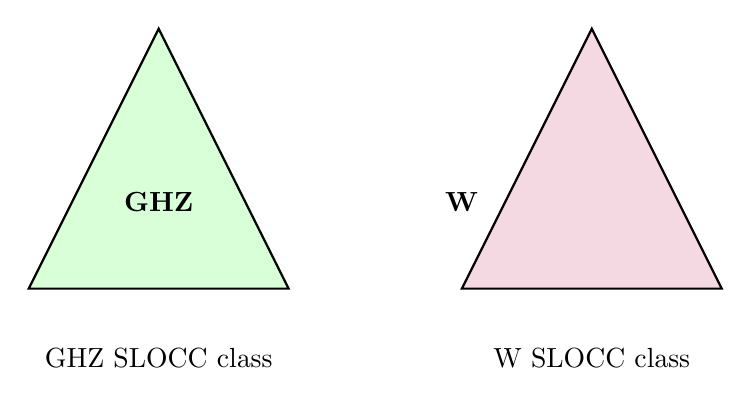
\begin{tikzpicture}[scale=1.1]
		\draw[thick, fill=green!15] (0,0) -- (3,0) -- (1.5,3) -- cycle;
		\node at (1.5,1) {\textbf{GHZ}};

		\draw[thick, fill=purple!15, xshift=5cm] (0,0) -- (3,0) -- (1.5,3) -- cycle;
		\node at (5,1) {\textbf{W}};

		\node at (1.5,-0.8) {GHZ SLOCC class};
		\node at (6.5,-0.8) {W SLOCC class};

	\end{tikzpicture}
	\caption{Three-qubit entanglement polytope showing the two tetrahedra corresponding to GHZ and W SLOCC classes. Each tetrahedron contains all states reachable within that SLOCC class, with product states at the vertices and maximally entangled states in the interior. Three-qubit entanglement polytope: For three qubits, the entanglement polytope consists of two tetrahedra corresponding to the GHZ and W SLOCC equivalence classes. States in different classes cannot be converted into each other by SLOCC operations.}
	\label{fig:entanglement-polytope-3qubit}
\end{figure}
